
Given equation can be written as
\begin{align}
      \label{quadform/51/eq1}
 x^2-4x-y+6 &=0
 \\
 \implies 
\vec{V}&=\myvec{1 & 0 \\ 0 & 0},\vec{u}=\myvec{2 \\ \frac{-1}{2}},f=6  \label{quadform/51/eq2}
\end{align}
Using eigen decomposition on $\vec{V}$,
\begin{align}
\vec{D}&= \myvec{0 & 0\\0 & 1}   \label{quadform/51/eq3}
\\
\vec{P}& =\myvec{0 & 1\\1 & 0}  \label{quadform/51/eq4}
\end{align}
The vertex of parabola $\vec{c}$ is given by
\begin{align}
\myvec{\vec{u}^T + \eta\vec{p_1}^T \\ \vec{V}}\vec{c} &= \myvec{-f \\ \eta\vec{p_1}-\vec{u}} \label{quadform/51/eq5}
\end{align}
\begin{align}
where,\eta=\vec{u}^T\vec{p_1}=\frac{-1}{2}  \label{quadform/51/eq6}
\end{align}
yielding
%Substituting values from \eqref{quadform/51/eq2},\eqref{quadform/51/eq4} and \eqref{quadform/51/eq6} in \eqref{quadform/51/eq5}
\begin{align}
\myvec{-2 & -1 \\ 1 & 0 \\ 0 & 0}\vec{c} &= \myvec{-6 \\ 2 \\ 0} \label{quadform/51/eq7}
\\
\implies \myvec{-2 & -1 & -6\\1 & 0 & 2} 
\xleftrightarrow{R_1\leftarrow \frac{R_1}{-2}}\myvec{1 & \frac{1}{2} & 2\\1 & 0 & 2} 
\\
%\myvec{1 & \frac{1}{2} & 3 \\0 & \frac{-1}{2} & -1}
\xleftrightarrow{R_2\leftarrow R_2 -R_1}\myvec{1 & \frac{1}{2} & 3 \\0 & \frac{-1}{2} & -1}
\\
%\myvec{1 & \frac{1}{2} & 3 \\0 & 1 & 2}
\xleftrightarrow{R_2\leftarrow (-2R_2)}\myvec{1 & \frac{1}{2} & 3 \\0 & 1 & 2}
\\
%\myvec{1 & 0 & 2\\0 & 1 & 2}
\implies \xleftrightarrow{R_1\leftarrow R_1 - \frac{R_2}{2}}\myvec{1 & 0 & 2\\0 & 1 & 2}   \label{quadform/51/eq8}
\end{align}
From $\eqref{quadform/51/eq8}$ it can be observed that,
\begin{align}
\vec{c} &= \myvec{2 \\ 2}
\\
\implies \vec{e_1}^T\vec{c}&=2  \quad\brak{\because\vec{e_1}=\myvec{1\\0}}
\end{align}
$\therefore$ From -$\infty$ to $\vec{e_1}^T\vec{c}$ the function is decreasing and from $\vec{e_1}^T\vec{c}$ to $\infty$ the function is increasing.
\begin{enumerate}
\item f is increasing in interval (2,$\infty$)
\item f is decreasing in interval (-$\infty$,2)
\end{enumerate}

This is verified in Fig.     \ref{quadform/51/fig:Prarabola}.
%
\begin{figure}[ht]
    \centering
    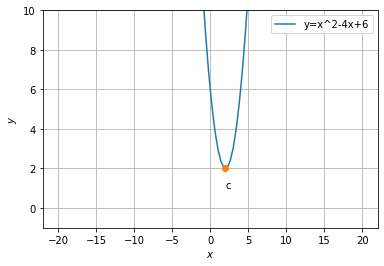
\includegraphics[width=\columnwidth]{solutions/su2021/2/51/Figure.png}
    \caption{Parabola}
    \label{quadform/51/fig:Prarabola}
\end{figure}    
